% Copyright (c) 2014,2016 Casper Ti. Vector
% Public domain.

\chapter{利用CNN分辨NLDBD事件和背景事件}
\label{chapter:cnn}

正如上文所述,NLDBD事件是一个及其稀有的事件,其半衰期超过了$1.07\times10^{26}$年,因而对于实验中的本底控制提出了很高的要求。根据第\ref{chapter:background}章所进行的背景模拟数据,PandaXIII实验中200kg级的探测器每年会探测到约78个本底$\gamma$事件落在ROI能量区间中,这个事件率还是远远高于实验的需求,因而需要一些其他的方式来压低本地信号,其中最自然的方法便是利用事件径迹的相关信息来区分背景事件和NLDBD事件。

NLDBD事件会同时释放出两个高能电子,在其径迹的两个末端会有这十分明显的布拉格峰,这是NLDBD事件最为明显的一个特征。而传统的$\gamma$本底事件一般通过一次或多次康普顿散射产生一个或多个次级电子,所以$\gamma$射线的径迹会形成一个或多个单末端布拉格峰的径迹。所以如果我们能够得到探测器探测到事件的详细径迹信息,就可以由此高效的分辨出本底事件和NLDBD事件,从而极大的压低本地。

然而因为PandaXIII读出系统的限制,使用传统的方法重建径迹会变得比较困难,因而我们探究了使用CNN深度神经网络来进行事件鉴别这一方法,得到了较为优异的效果。本章节详细描述了利用CNN进行事件鉴别的动机,CNN模型的选择和搭建,数据处理和训练等细节,希望能够帮助读者建立起对于CNN清晰简单的认识,为高能物理研究甚至是其他领域的研究提供相应的帮助。

\section{传统鉴别方法以及遇到的困难}

如前文所述,NLDBD是一个径迹特征即为明显的事件,该特征能够极大地帮助实验的进行。图\ref{fig:samples}给出了NLDBD和背景事件的对比,可以很明显的看出NLDBD事件径迹在末端拥有两个明显的布拉格峰,而背景$\gamma$事件则只存在一个布拉格峰。如果我们的TPC能够完美的重建出事件的径迹信息,那么鉴别该事件是否是NLDBD事件就会变得及其的简单:llin2018designin2018design我们只要重建出径迹沉积的能量随径迹位置的关系,然后使用简单的cut就可以判断该事件的类型。然而在PandaXIII中重建径迹这个操作是十分困难的,原因如下。

\begin{figure}[hbt]
    \centering
    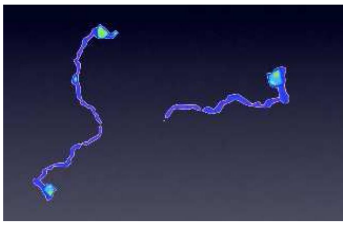
\includegraphics[width=0.5\columnwidth]{pic/fig10.png}
    \caption{一个NLDBD事件(左图)和一个$\gamma$背景事件(右图)径迹投影图。可以很明显的分辨出左侧径迹末端有两个布拉格峰,而右侧只有一个末端有布拉格峰。}
    \label{fig:samples}
\end{figure}

PandaXIII设计使用了41个Microbulk Micromegas读出板来构建读出平面,每个MM(Microbulk Micromegas)板的尺寸为20厘米x20厘米,按照图\ref{fig:mms}所示的形状排列组成,这样的话读出平面能够极大的覆盖漂移区域,从而提升事件的探测效率。

\begin{figure}[hbt]
    \centering
    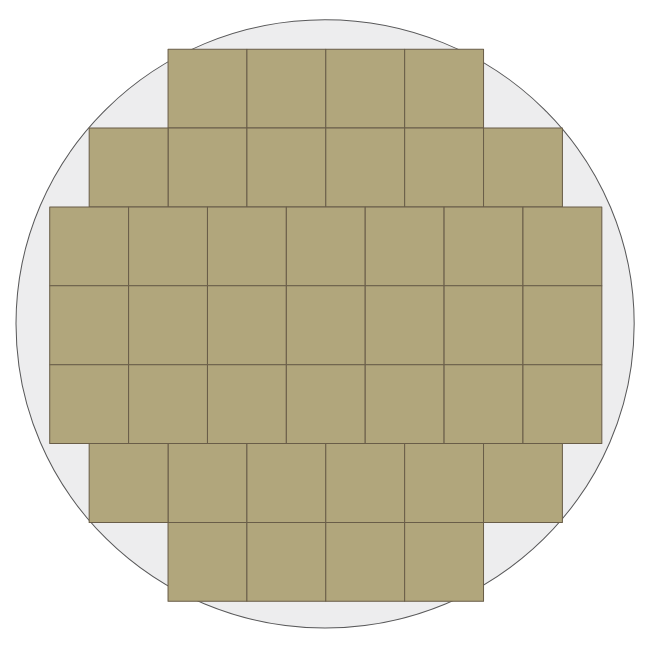
\includegraphics[width=0.4\columnwidth]{pic/fig8.png}
    \caption{41个MM板组合探测器读出平面排放示意图,按照4,6,7,7,7,6,4层叠放置。}
    \label{fig:mms}
\end{figure}

如图\ref{fig:mm_detail}左图所示,每个MM上都密布了许多增益孔(Amplification holes),用于采集漂移到附近的电子。这些增益孔按照合适的排布组成菱形的读出像素,每个像素的对角线尺寸约为3毫米,这边是Micromegas的位置分辨率。如果MM采取像素读出的话,一块MM会拥有约4000个通道(channel),整个TPC则会超过32万,这么多道数对于电子学部分基本是不可以承受的,因而PandaXIII使用了条状读出,而不是像素读出。如图\ref{fig:mm_detail}右图所示,每一组红色像素被连接在一起,在Y方向上形成64个通道,X方向上同样由黄色像素组成64个通道。这样的话一块MM读出板只会形成128个通道,从而大大降低了电子学的复杂程度。

\begin{figure}
    \centering
    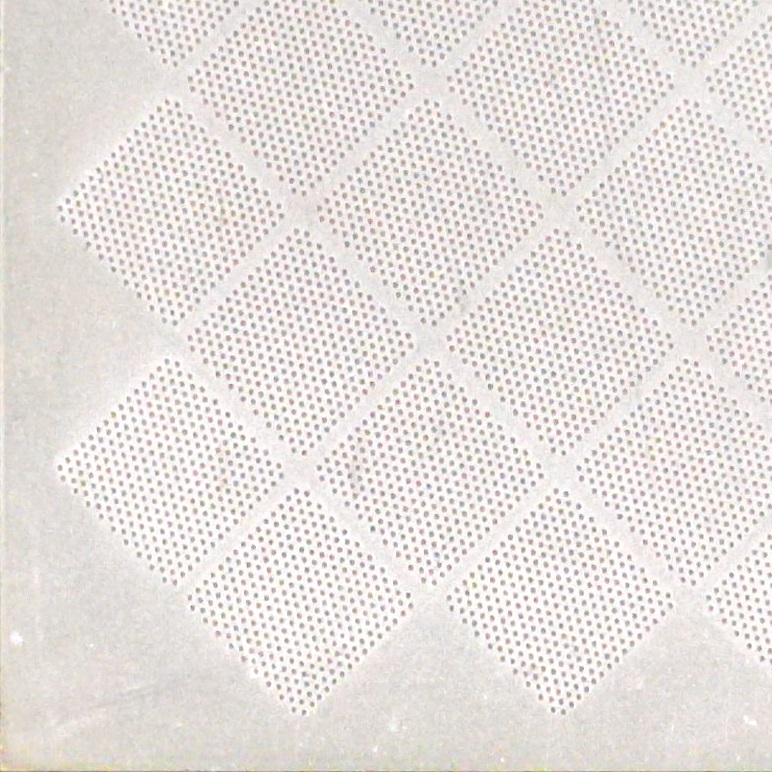
\includegraphics[width=0.4\columnwidth]{pic/MMStrips.jpg}
    \includegraphics[width=0.4\columnwidth]{pic/MMPattern.pdf}
    \caption{左图,MM板局部读出区域的放大示意图,图中的小孔便是增益孔(Amplification Holes),若干孔组成一个菱形读出像素,每个像素的对角线长度约为3毫米。右图:MM板局部读出通道(channel)连接示意图,红色以及黄色菱形(正方形)区域即为中图所示的读出像素,每一条红色虚线或者黄色虚线连接了一组读出像素,形成一个读出通道。\supercite{lin2018design}}
    \label{fig:mm_detail}
\end{figure}

但是采取条状读出也有对应的弊端,即我们无法同时获取到漂移到MM读出板上电子的X和Y的位置,我们只能得到它的X\textbf{或}Y的位置。再加上通过漂移时间计算得到的Z轴相对位置关系后,我们能够轻易的得到一个事件的X-Z-energy投影信息和Y-Z-energy投影信息,而有关X-Y的信息则因为MM结构问题而被彻底抹去了,这就使得重建径迹的3维信息变得极其的困难。

虽然一条比较直的径迹可以紧紧通过X-Z以及Y-Z来组合得到X-Y-Z的径迹,但是电子在TPC中的运动径迹往往不规则,同一时刻往往会有超过一组X和Y读出条被触发,这样同一Z值(同一时刻)的XY信息就无法确定,如图\ref{fig:difficulty_track_2}所示。如果两个真实的hit分别位于($x_1$,$y_1$)和($x_2$,$y_2$),那么因为条状读出的原因,$x_1,x_2,y_1,y_2$所在的通道会同时被触发,那么重建就可能得到错误的能量沉积点。图\ref{fig:difficulty_track}便给出了一个难于重建的
NLDBD事件投影图,该事件在Z在(80,110)毫米处的径迹纠缠在了一起,所以基本上不可能完成重建。

\begin{figure}
    \centering
    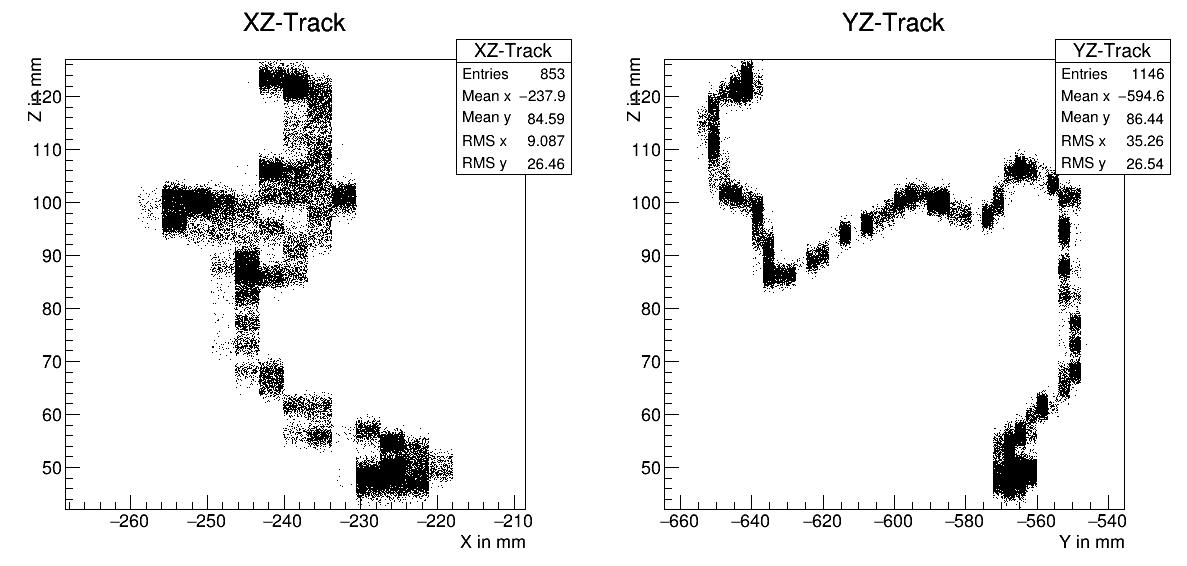
\includegraphics[width=0.7\columnwidth]{pic/difficulty_track.png}
    \caption{一个难于重建的事件的XZ投影和YZ投影,区块深浅表示沉积能量的大小,Z在(80,110)毫米内的径迹因为X方向上的多种可能而变得无法重建。}
    \label{fig:difficulty_track}
\end{figure}

\begin{figure}
    \centering
    \includegraphics[width=0.3\columnwidth]{pic/app01_strip_readout.pdf}
    \caption{条状读出易混淆的示意图。真实的能量沉积位置如图中绿色点所示($x_1$,$y_1$)和($x_2$,$y_2$),但是因为$x_1,x_2,y_1,y_2$所在的通道同时被触发,因而可能得到红色表示的错误重建结果。}
    \label{fig:difficulty_track_2}
\end{figure}

MM条状读出同时还带来了另外一个困难,因为一个电子要么落在X读出条所在的像素中,要么落在Y读出条所在的像素中,因而径迹相同位置在重建后的两个投影处的能量并不相等。所以根据能量的大小做X-Y的匹配也困难重重。作者个人认为在使用MM条状读出的前提下,能够良好的重建出径迹基本是不可能的,因而需要探寻新型的事件鉴别的方式方法。于是我们便试图将近年来在计算机领域大放异彩的深度神经网络引入我们的粒子鉴别,以期望它能够解决这个难题。

\section{CNN介绍以及使用动机}

正如上文所说的,虽然

\section{数据准备和训练}

\subsection{读出平面的结构}


\section{测试结果分析}
% vim:ts=4:sw=4
